% Final viva deck. Every number is a macro from ../generated/{results,final}.tex, built by
% ../build_final.py from results/final/, so the slides cannot drift from the report.
% Build: bash ../build_slides.sh  (pdflatex + beamer)
\documentclass[aspectratio=169,11pt]{beamer}
\usetheme{default}
\usecolortheme{dove}
\setbeamertemplate{navigation symbols}{}
\setbeamertemplate{footline}[frame number]
\usepackage{lmodern}
\usepackage[T1]{fontenc}
\usepackage{booktabs}
\usepackage{graphicx}
\usepackage{amsmath}
\IfFileExists{adjustbox.sty}{\usepackage{adjustbox}}{%
  \newsavebox{\escapebox}%
  \newenvironment{adjustbox}[1]{\begin{lrbox}{\escapebox}}%
    {\end{lrbox}\ifdim\wd\escapebox>\linewidth\resizebox{\linewidth}{!}{\usebox{\escapebox}}\else\usebox{\escapebox}\fi}}
\graphicspath{{../}{../../../}}
% Generated by reports/mid_submission/build_results.py -- do not edit by hand.
% Source run: results/final/c-v1-2721954
\providecommand{\textcolor}[2]{#2}
\newcommand{\BppCpp}{7.86}
\newcommand{\BppEn}{3.77}
\newcommand{\BppPy}{5.68}
\newcommand{\BppSdCpp}{3.10}
\newcommand{\BppSdEn}{0.52}
\newcommand{\BppSdPy}{1.61}
\newcommand{\BppVarCpp}{527.8}
\newcommand{\BppVarEn}{10.3}
\newcommand{\BppVarPy}{69.4}
\newcommand{\DetMarginCpp}{+0.691}
\newcommand{\DetMarginPy}{+0.759}
\newcommand{\EndMarginCpp}{-0.035}
\newcommand{\EndMarginEn}{-0.079}
\newcommand{\EndMarginPy}{-0.017}
\newcommand{\FidelityAda}{passed}
\newcommand{\FoneCpp}{0.165}
\newcommand{\FoneEn}{0.495}
\newcommand{\FoneNullCpp}{0.036}
\newcommand{\FoneNullEn}{0.147}
\newcommand{\FoneNullPy}{0.032}
\newcommand{\FonePy}{0.152}
\newcommand{\IouBltCpp}{0.372}
\newcommand{\IouBltEn}{0.377}
\newcommand{\IouBltPy}{0.351}
\newcommand{\IouLineCpp}{0.606}
\newcommand{\IouLineEn}{0.049}
\newcommand{\IouLinePy}{0.546}
\newcommand{\IouNullCpp}{0.356}
\newcommand{\IouNullEn}{0.334}
\newcommand{\IouNullPy}{0.342}
\newcommand{\IouResamples}{100}
\newcommand{\IouVsNullCICpp}{[0.013, 0.018]}
\newcommand{\IouVsNullCIEn}{[0.040, 0.045]}
\newcommand{\IouVsNullCIPy}{[0.007, 0.010]}
\newcommand{\IouVsNullCpp}{+0.016}
\newcommand{\IouVsNullEn}{+0.042}
\newcommand{\IouVsNullPy}{+0.008}
\newcommand{\IouWordCpp}{0.409}
\newcommand{\IouWordEn}{0.397}
\newcommand{\IouWordPy}{0.342}
\newcommand{\MarginCICpp}{[0.125, 0.134]}
\newcommand{\MarginCIEn}{[0.341, 0.354]}
\newcommand{\MarginCIPy}{[0.117, 0.122]}
\newcommand{\MarginCode}{+0.129}
\newcommand{\MarginCpp}{+0.129}
\newcommand{\MarginEn}{+0.348}
\newcommand{\MarginProse}{+0.348}
\newcommand{\MarginPy}{+0.120}
\newcommand{\OFive}{a positive residual}
\newcommand{\OFiveEligible}{2,902}
\newcommand{\OFiveFiles}{1,500}
\newcommand{\OFiveInference}{OLS with file-cluster robust covariance; t intervals}
\newcommand{\OFiveRegions}{12,609}
\newcommand{\OFiveUnsafe}{+6.93e-03}
\newcommand{\OFiveUnsafeCI}{[0.0043, 0.0095]}
\newcommand{\OFourCaseRate}{50\%}
\newcommand{\OFourCleanCpp}{+0.131}
\newcommand{\OFourCleanPy}{+0.115}
\newcommand{\OFourDbppCppCase}{-0.10}
\newcommand{\OFourDbppCppIndent}{-0.13}
\newcommand{\OFourDbppCppSemi}{-0.06}
\newcommand{\OFourDbppCppTypo}{-0.34}
\newcommand{\OFourDbppPyCase}{-0.05}
\newcommand{\OFourDbppPyIndent}{+0.004}
\newcommand{\OFourDbppPyTypo}{-0.23}
\newcommand{\OFourFiles}{1,000}
\newcommand{\OFourMinMarginCpp}{+0.118}
\newcommand{\OFourMinMarginPy}{+0.099}
\newcommand{\OFourPerm}{1,000}
\newcommand{\OFourRate}{20\%}
\newcommand{\OFourWorstCpp}{indentation}
\newcommand{\OFourWorstDmCICpp}{[-0.015, -0.012]}
\newcommand{\OFourWorstDmCIPy}{[-0.018, -0.015]}
\newcommand{\OFourWorstDmCpp}{-0.013}
\newcommand{\OFourWorstDmPy}{-0.016}
\newcommand{\OFourWorstPy}{indentation}
\newcommand{\OpenMarginCpp}{+0.451}
\newcommand{\OpenMarginPy}{+0.611}
\newcommand{\PFourAll}{is larger in both code languages}
\newcommand{\PFourCpp}{not smaller}
\newcommand{\PFourPy}{not smaller}
\newcommand{\PFourSupported}{do not support}
\newcommand{\POneAll}{exceeds the null in all three languages}
\newcommand{\POneCpp}{exceeds}
\newcommand{\POneEn}{exceeds}
\newcommand{\POnePy}{exceeds}
\newcommand{\PThree}{not larger}
\newcommand{\PThreeCmp}{smaller than}
\newcommand{\PTwoAll}{exceeds the end margin in all three languages}
\newcommand{\PTwoCpp}{larger}
\newcommand{\PTwoEn}{larger}
\newcommand{\PTwoPy}{larger}
\newcommand{\PrecCpp}{0.095}
\newcommand{\PrecEn}{0.342}
\newcommand{\PrecPy}{0.083}
\newcommand{\PrecRecAll}{is below recall in all three languages}
\newcommand{\PrecRecCpp}{below}
\newcommand{\PrecRecEn}{below}
\newcommand{\PrecRecPy}{below}
\newcommand{\PvalCpp}{$\leq$1e-4}
\newcommand{\PvalEn}{$\leq$1e-4}
\newcommand{\PvalPy}{$\leq$1e-4}
\newcommand{\RTwoAll}{underperforms it in all three languages}
\newcommand{\RTwoCpp}{underperforms}
\newcommand{\RTwoEn}{underperforms}
\newcommand{\RTwoPy}{underperforms}
\newcommand{\RecCpp}{0.646}
\newcommand{\RecEn}{0.894}
\newcommand{\RecPy}{0.822}
\newcommand{\StrongestCpp}{word-start}
\newcommand{\StrongestEn}{word-start}
\newcommand{\StrongestFoneCpp}{0.339}
\newcommand{\StrongestFoneEn}{0.769}
\newcommand{\StrongestFonePy}{0.394}
\newcommand{\StrongestPy}{indentation}
\newcommand{\VsBaseCICpp}{[-0.181, -0.167]}
\newcommand{\VsBaseCIEn}{[-0.280, -0.268]}
\newcommand{\VsBaseCIPy}{[-0.247, -0.237]}
\newcommand{\VsBaseCpp}{-0.173}
\newcommand{\VsBaseEn}{-0.274}
\newcommand{\VsBasePy}{-0.242}
\newcommand{\kCpp}{0}
\newcommand{\kEn}{0}
\newcommand{\kPy}{0}
\newcommand{\nBoot}{2,000}
\newcommand{\nCalCpp}{1,600}
\newcommand{\nCalEn}{60}
\newcommand{\nCalPy}{1,600}
\newcommand{\nExtracted}{16,300}
\newcommand{\nPerm}{10,000}
\newcommand{\nSamples}{16,300}
\newcommand{\nTestAll}{13,040}
\newcommand{\nTestCpp}{6,400}
\newcommand{\nTestEn}{240}
\newcommand{\nTestPy}{6,400}
\newcommand{\TableMain}{
\begin{table*}[t]\centering\small

\begin{adjustbox}{max width=\textwidth}\begin{tabular}{lrrrrrrlr}\toprule
Language & $k$ & Test files & P & R & F1 & $H_0$ F1 & $\Delta$F1 [95\% CI] & $p$ \\\midrule
Python & 0 & 6,400 & 0.083 & 0.822 & 0.152 & 0.032 & +0.120 [0.117, 0.122] & $\leq$1e-4 \\
C++ & 0 & 6,400 & 0.095 & 0.646 & 0.165 & 0.036 & +0.129 [0.125, 0.134] & $\leq$1e-4 \\
English & 0 & 240 & 0.342 & 0.894 & 0.495 & 0.147 & +0.348 [0.341, 0.354] & $\leq$1e-4 \\
\bottomrule\end{tabular}\end{adjustbox}
\caption{Held-out entropy-boundary alignment with constituent starts (P1). $k$ was frozen on the calibration split. $H_0$ F1 is the permutation mean of the fixed-EOF density-matched null (10,000 permutations); intervals are paired file bootstraps; $p$ is the one-sided permutation value.}
\label{tab:main}\end{table*}}
\newcommand{\TableBaselines}{
\begin{table}[t]\centering\small

\begin{adjustbox}{max width=\columnwidth}\begin{tabular}{lrrrrl}\toprule
Lang. & BLT & NL & Indent & Word & BLT$-$best [95\% CI] \\\midrule
Python & 0.152 & 0.000 & 0.394 & 0.245 & -0.242 [-0.247, -0.237] \\
C++ & 0.165 & 0.041 & 0.281 & 0.339 & -0.173 [-0.181, -0.167] \\
English & 0.495 & 0.000 & 0.008 & 0.769 & -0.274 [-0.280, -0.268] \\
\bottomrule\end{tabular}\end{adjustbox}
\caption{Start F1 of structure-blind baselines under the same targets, $k$ and matching: boundary after every newline (NL), at indentation changes, and at every word start. The last column compares BLT with the strongest baseline for that language. Newline scores 0 in Python because the byte after a newline is indentation, never a start at $k=0$; English paragraphs contain no newline.}
\label{tab:baselines}\end{table}}
\newcommand{\TableStartEnd}{
\begin{table}[t]\centering\small

\begin{adjustbox}{max width=\columnwidth}\begin{tabular}{lrrrrrl}\toprule
 & \multicolumn{3}{c}{Starts} & \multicolumn{3}{c}{Ends} \\
Lang. & R & F1 & $\Delta$ & R & F1 & $\Delta$ [95\% CI] \\\midrule
Python & 0.822 & 0.152 & +0.120 & 0.034 & 0.004 & -0.017 [-0.017, -0.016] \\
C++ & 0.646 & 0.165 & +0.129 & 0.026 & 0.008 & -0.035 [-0.036, -0.034] \\
English & 0.894 & 0.495 & +0.348 & 0.066 & 0.026 & -0.079 [-0.081, -0.076] \\
\bottomrule\end{tabular}\end{adjustbox}
\caption{Starts versus ends (P2). $\Delta$ is F1 minus the mean $H_0$ F1.}
\label{tab:startend}\end{table}}
\newcommand{\TableTypes}{
\begin{table}[t]\centering\small

\begin{adjustbox}{max width=\columnwidth}\begin{tabular}{llcrrrr}\toprule
Lang. & Type & Opener & Starts & R & $H_0$ R & $\Delta$R \\\midrule
Python & \texttt{assignment} & open & 39 & 0.872 & 0.156 & +0.715 \\
Python & \texttt{binary\_operator} & open & 7,276 & 0.683 & 0.184 & +0.498 \\
Python & \texttt{call} & open & 33,643 & 0.766 & 0.168 & +0.598 \\
Python & \texttt{expression\_statement} & open & 43,709 & 0.864 & 0.169 & +0.695 \\
Python & \texttt{for\_statement} & det. & 2,829 & 0.934 & 0.162 & +0.772 \\
Python & \texttt{function\_definition} & det. & 485 & 0.891 & 0.166 & +0.724 \\
Python & \texttt{if\_statement} & det. & 10,084 & 0.903 & 0.158 & +0.745 \\
Python & \texttt{return\_statement} & open & 7,010 & 0.798 & 0.249 & +0.550 \\
Python & \texttt{while\_statement} & det. & 263 & 0.954 & 0.161 & +0.794 \\
C++ & \texttt{assignment\_expression} & open & 8,078 & 0.452 & 0.133 & +0.319 \\
C++ & \texttt{binary\_expression} & open & 285,064 & 0.506 & 0.144 & +0.362 \\
C++ & \texttt{call\_expression} & open & 456,491 & 0.595 & 0.138 & +0.457 \\
C++ & \texttt{declaration} & open & 249,479 & 0.773 & 0.142 & +0.632 \\
C++ & \texttt{expression\_statement} & open & 486,954 & 0.655 & 0.138 & +0.517 \\
C++ & \texttt{for\_statement} & det. & 21,326 & 0.823 & 0.136 & +0.686 \\
C++ & \texttt{function\_definition} & det. & 101,613 & 0.768 & 0.134 & +0.635 \\
C++ & \texttt{if\_statement} & det. & 126,003 & 0.795 & 0.146 & +0.649 \\
C++ & \texttt{return\_statement} & open & 93,611 & 0.562 & 0.144 & +0.418 \\
C++ & \texttt{while\_statement} & det. & 4,102 & 0.942 & 0.150 & +0.792 \\
\bottomrule\end{tabular}\end{adjustbox}
\caption{Start recall by constituent type (P4). Types are rematched separately, so rows are not additive. A start shared by several nodes is credited to the outermost one, which is why nested types such as Python \texttt{assignment} have few starts. Opener class follows the empirically checked \texttt{taxonomy.json}.}
\label{tab:types}\end{table}}
\newcommand{\TableIoU}{
\begin{table}[t]\centering\small

\begin{adjustbox}{max width=\columnwidth}\begin{tabular}{lrrrrrl}\toprule
Lang. & Files & BLT & $H_0$ & Line & Word & BLT$-H_0$ [95\% CI] \\\midrule
Python & 6,400 & 0.351 & 0.342 & 0.546 & 0.342 & +0.008 [0.007, 0.010] \\
C++ & 6,188 & 0.372 & 0.356 & 0.606 & 0.409 & +0.016 [0.013, 0.018] \\
English & 240 & 0.377 & 0.334 & 0.049 & 0.397 & +0.042 [0.040, 0.045] \\
\bottomrule\end{tabular}\end{adjustbox}
\caption{Secondary metric: mean best single-patch IoU over unique constituent spans, held-out split (files with at least one span). $H_0$ averages 100 fixed-EOF permutations; Line and Word are newline and word-start segmentations.}
\label{tab:iou}\end{table}}
\newcommand{\TableOFour}{
\begin{table*}[t]\centering\small

\begin{adjustbox}{max width=\textwidth}\begin{tabular}{llrrlrl}\toprule
Lang. & Noise & Edits & $\Delta$F1 vs.\ $H_0$ & Change vs.\ clean [95\% CI] & BPP & Change vs.\ clean [95\% CI] \\\midrule
Python & clean & 0 & +0.115 & -- & 5.61 & -- \\
Python & camel$\leftrightarrow$snake & 4,601 & +0.114 & -0.001 [-0.002, -0.001] & 5.56 & -0.05 [-0.06, -0.04] \\
Python & indentation & 4,416 & +0.099 & -0.016 [-0.018, -0.015] & 5.61 & +0.004 [-0.003, 0.010] \\
Python & keyword typo & 1,626 & +0.112 & -0.003 [-0.004, -0.003] & 5.38 & -0.23 [-0.25, -0.21] \\
C++ & clean & 0 & +0.131 & -- & 7.88 & -- \\
C++ & camel$\leftrightarrow$snake & 83,037 & +0.129 & -0.002 [-0.003, -0.002] & 7.78 & -0.10 [-0.11, -0.09] \\
C++ & indentation & 68,746 & +0.118 & -0.013 [-0.015, -0.012] & 7.75 & -0.13 [-0.14, -0.12] \\
C++ & keyword typo & 17,884 & +0.131 & -0.0004 [-0.0010, 0.0001] & 7.54 & -0.34 [-0.36, -0.31] \\
C++ & missing \texttt{;} & 25,972 & +0.129 & -0.002 [-0.002, -0.002] & 7.82 & -0.06 [-0.06, -0.05] \\
\bottomrule\end{tabular}\end{adjustbox}
\caption{Objective 4: robustness to code noise on 1,000 held-out test files per language (so the clean margin differs slightly from Table~\ref{tab:main}). Each noise type is applied alone; targets are the clean constituents mapped to noised offsets; $k$ is the frozen value. The null uses 1,000 fixed-EOF permutations per file; intervals are paired file bootstraps of noised minus clean.}
\label{tab:o4}\end{table*}}
\newcommand{\TableOFive}{
\begin{table}[t]\centering\small

\begin{adjustbox}{max width=\columnwidth}\begin{tabular}{llrlr}\toprule
Outcome & Term & Coef. & 95\% CI & $p$ \\\midrule
boundary density & memory-unsafe & +6.93e-03 & [0.0043, 0.0095] & 0.000 \\
boundary density & identifier entropy (nats) & +2.51e-01 & [0.2422, 0.2590] & 0.000 \\
boundary density & identifier byte share & +8.77e-03 & [-0.0021, 0.0196] & 0.114 \\
boundary density & region length (bytes) & -2.40e-05 & [-4.42e-05, -3.82e-06] & 0.020 \\
inverse BPP & memory-unsafe & +1.12e-02 & [0.0087, 0.0137] & 0.000 \\
inverse BPP & identifier entropy (nats) & +2.31e-01 & [0.2227, 0.2402] & 0.000 \\
inverse BPP & identifier byte share & +2.45e-02 & [0.0142, 0.0347] & 0.000 \\
inverse BPP & region length (bytes) & -7.70e-06 & [-1.54e-05, -5.25e-08] & 0.048 \\
\bottomrule\end{tabular}\end{adjustbox}
\caption{O5 region regressions with file fixed effects and statement-type controls; file-clustered intervals.}
\label{tab:o5}\end{table}}

% Generated by reports/final_submission/build_final.py -- do not edit by hand.
\newcommand{\xAdaptBpb}{1.09}
\newcommand{\xAdaptDiffCICpp}{[0.003, 0.007]}
\newcommand{\xAdaptDiffCIEn}{[0.026, 0.032]}
\newcommand{\xAdaptDiffCIPy}{[0.004, 0.008]}
\newcommand{\xAdaptDiffCpp}{+0.005}
\newcommand{\xAdaptDiffEn}{+0.029}
\newcommand{\xAdaptDiffPy}{+0.006}
\newcommand{\xAdaptRefWinFone}{0.871}
\newcommand{\xAdaptRefWinFoneCpp}{0.880}
\newcommand{\xAdaptRefWinFoneProse}{0.834}
\newcommand{\xAdaptRefWinFonePy}{0.869}
\newcommand{\xAdaptVerdict}{not met}
\newcommand{\xAdaptVsBaseCpp}{-0.117}
\newcommand{\xAdaptVsBaseEn}{-0.287}
\newcommand{\xAdaptVsBasePy}{-0.243}
\newcommand{\xAdaptWidthCpp}{0.022}
\newcommand{\xAdaptWidthEn}{0.013}
\newcommand{\xAdaptWidthPy}{0.017}
\newcommand{\xAdaptWinFone}{0.955}
\newcommand{\xAdaptWinFoneCpp}{0.958}
\newcommand{\xAdaptWinFoneProse}{0.937}
\newcommand{\xAdaptWinFonePy}{0.955}
\newcommand{\xAdaptWins}{1}
\newcommand{\xAlphaBpb}{1.17}
\newcommand{\xAlphaFone}{0.789}
\newcommand{\xAlphaFoneCpp}{0.791}
\newcommand{\xAlphaFoneProse}{0.764}
\newcommand{\xAlphaFonePy}{0.798}
\newcommand{\xArmsNCpp}{300}
\newcommand{\xArmsNEn}{240}
\newcommand{\xArmsNPy}{300}
\newcommand{\xAuditAgree}{433/435}
\newcommand{\xAuditRepro}{12,609/12,609}
\newcommand{\xBalBpb}{1.27}
\newcommand{\xBalDiffCICpp}{[-0.0035, -0.0001]}
\newcommand{\xBalDiffCIEn}{[0.008, 0.012]}
\newcommand{\xBalDiffCIPy}{[-0.003, -0.001]}
\newcommand{\xBalDiffCpp}{-0.002}
\newcommand{\xBalDiffEn}{+0.010}
\newcommand{\xBalDiffPy}{-0.002}
\newcommand{\xBalRefWinFone}{0.871}
\newcommand{\xBalRefWinFoneCpp}{0.880}
\newcommand{\xBalRefWinFoneProse}{0.834}
\newcommand{\xBalRefWinFonePy}{0.869}
\newcommand{\xBalVsBaseCpp}{-0.124}
\newcommand{\xBalVsBaseEn}{-0.302}
\newcommand{\xBalVsBasePy}{-0.251}
\newcommand{\xBalWinFone}{0.860}
\newcommand{\xBalWinFoneCpp}{0.860}
\newcommand{\xBalWinFoneProse}{0.853}
\newcommand{\xBalWinFonePy}{0.864}
\newcommand{\xDepthOneCpp}{+0.553}
\newcommand{\xDepthOneEn}{+0.714}
\newcommand{\xDepthOnePy}{+0.707}
\newcommand{\xDepthSevenCpp}{+0.387}
\newcommand{\xDepthSevenEn}{+0.601}
\newcommand{\xDepthSevenPy}{+0.519}
\newcommand{\xDistBpb}{1.24}
\newcommand{\xDistFone}{0.871}
\newcommand{\xDistFoneCpp}{0.880}
\newcommand{\xDistFoneProse}{0.834}
\newcommand{\xDistFonePy}{0.869}
\newcommand{\xEffForward}{5.0}
\newcommand{\xEffGpu}{RTX 2080 Ti}
\newcommand{\xEffNative}{13,246}
\newcommand{\xEffRolling}{4.8}
\newcommand{\xErrDiff}{+0.004}
\newcommand{\xErrDiffCI}{[-0.005, 0.015]}
\newcommand{\xErrShare}{28.0\%}
\newcommand{\xFileCI}{[0.118, 0.122]}
\newcommand{\xGateMaxDev}{0.0000}
\newcommand{\xHfDiffCICpp}{[-0.126, -0.121]}
\newcommand{\xHfDiffCIEn}{[-0.211, -0.183]}
\newcommand{\xHfDiffCIPy}{[-0.099, -0.095]}
\newcommand{\xHfDiffCpp}{-0.123}
\newcommand{\xHfDiffEn}{-0.198}
\newcommand{\xHfDiffPy}{-0.097}
\newcommand{\xHfMarginCpp}{+0.008}
\newcommand{\xHfMarginEn}{+0.150}
\newcommand{\xHfMarginPy}{+0.023}
\newcommand{\xHfNCpp}{4,384}
\newcommand{\xHfNEn}{240}
\newcommand{\xHfNPy}{6,400}
\newcommand{\xHfSwaMarginCpp}{+0.131}
\newcommand{\xHfSwaMarginEn}{+0.348}
\newcommand{\xHfSwaMarginPy}{+0.120}
\newcommand{\xHfVsBaseCpp}{-0.252}
\newcommand{\xHfVsBaseEn}{-0.450}
\newcommand{\xHfVsBasePy}{-0.339}
\newcommand{\xHoldFiles}{4,107}
\newcommand{\xHoldStuFone}{0.463}
\newcommand{\xHoldStuMargin}{+0.305}
\newcommand{\xHoldStuVsWord}{-0.311}
\newcommand{\xHoldStuVsWordCI}{[-0.312, -0.310]}
\newcommand{\xHoldTargets}{317,378}
\newcommand{\xHoldTeaFone}{0.500}
\newcommand{\xHoldTeaMargin}{+0.350}
\newcommand{\xHoldTeaVsWord}{-0.273}
\newcommand{\xHoldTeaVsWordCI}{[-0.275, -0.272]}
\newcommand{\xHoldWord}{0.774}
\newcommand{\xKwDetCICpp}{[-0.092, -0.085]}
\newcommand{\xKwDetCIPy}{[-0.133, -0.127]}
\newcommand{\xKwDetCpp}{-0.088}
\newcommand{\xKwDetPy}{-0.130}
\newcommand{\xKwOpenCICpp}{[-0.054, -0.046]}
\newcommand{\xKwOpenCIPy}{[-0.068, -0.063]}
\newcommand{\xKwOpenCpp}{-0.050}
\newcommand{\xKwOpenPy}{-0.065}
\newcommand{\xKwRateDetCpp}{0.048}
\newcommand{\xKwRateDetPy}{0.029}
\newcommand{\xKwRateOpenCpp}{0.087}
\newcommand{\xKwRateOpenPy}{0.094}
\newcommand{\xLongBytes}{86\%}
\newcommand{\xLongDiff}{-0.002}
\newcommand{\xLongDiffCI}{[-0.008, 0.004]}
\newcommand{\xLongShare}{31.5\%}
\newcommand{\xNextDetCICpp}{[0.013, 0.029]}
\newcommand{\xNextDetCIPy}{[0.728, 0.743]}
\newcommand{\xNextDetCpp}{+0.021}
\newcommand{\xNextDetPy}{+0.736}
\newcommand{\xNextIfCpp}{-0.144}
\newcommand{\xNextIfPy}{+0.719}
\newcommand{\xNextOpenCICpp}{[0.089, 0.110]}
\newcommand{\xNextOpenCIPy}{[-0.004, 0.002]}
\newcommand{\xNextOpenCpp}{+0.101}
\newcommand{\xNextOpenPy}{-0.001}
\newcommand{\xNextRateDetCpp}{0.161}
\newcommand{\xNextRateDetPy}{0.895}
\newcommand{\xNextRateOpenCpp}{0.241}
\newcommand{\xNextRateOpenPy}{0.178}
\newcommand{\xOFiveCheck}{reproduces}
\newcommand{\xOFiveFull}{+0.0069}
\newcommand{\xOFiveFullCI}{[0.0043, 0.0095]}
\newcommand{\xOFiveRaw}{-0.0083}
\newcommand{\xOFiveRawCI}{[-0.0127, -0.0039]}
\newcommand{\xOFiveRel}{4.2\%}
\newcommand{\xOFiveRelBpp}{7.5\%}
\newcommand{\xOFiveSafeMean}{0.166}
\newcommand{\xOFiveUnsafeMean}{0.155}
\newcommand{\xOFiveVsIdent}{7\%}
\newcommand{\xOFourCaseMaxCpp}{-0.002}
\newcommand{\xOFourCaseMaxPy}{-0.001}
\newcommand{\xOFourIndentHiCpp}{-0.023}
\newcommand{\xOFourIndentHiPy}{-0.029}
\newcommand{\xOFourIndentLoCpp}{-0.004}
\newcommand{\xOFourIndentLoPy}{-0.005}
\newcommand{\xOFourSweepFiles}{1,000}
\newcommand{\xOFourSweepMinMargin}{+0.086}
\newcommand{\xOFourSweepWorst}{indentation at rate 0.4 in Python (-0.029)}
\newcommand{\xOFourTypoBppCpp}{-0.60}
\newcommand{\xOFourTypoBppPy}{-0.43}
\newcommand{\xOFourTypoHiCpp}{-0.002}
\newcommand{\xOFourTypoHiPy}{-0.007}
\newcommand{\xOffDetCppI}{0.039}
\newcommand{\xOffDetCppII}{0.016}
\newcommand{\xOffDetCppIII}{0.053}
\newcommand{\xOffDetCppIV}{0.377}
\newcommand{\xOffDetPyI}{0.035}
\newcommand{\xOffDetPyII}{0.003}
\newcommand{\xOffDetPyIII}{0.650}
\newcommand{\xOffDetPyIV}{0.300}
\newcommand{\xOffNullCpp}{0.140}
\newcommand{\xOffNullPy}{0.159}
\newcommand{\xPosCheck}{reproduce}
\newcommand{\xPostKwDetCICpp}{[-0.109, -0.102]}
\newcommand{\xPostKwDetCIPy}{[-0.161, -0.157]}
\newcommand{\xPostKwDetCpp}{-0.105}
\newcommand{\xPostKwDetPy}{-0.159}
\newcommand{\xPostKwOpenCICpp}{[-0.006, 0.003]}
\newcommand{\xPostKwOpenCIPy}{[-0.017, -0.010]}
\newcommand{\xPostKwOpenCpp}{-0.001}
\newcommand{\xPostKwOpenPy}{-0.014}
\newcommand{\xPostKwRateDetCpp}{0.035}
\newcommand{\xPostKwRateDetPy}{0.000}
\newcommand{\xPostKwRateOpenCpp}{0.139}
\newcommand{\xPostKwRateOpenPy}{0.156}
\newcommand{\xPostKwReturnCpp}{-0.139}
\newcommand{\xPostKwReturnPy}{-0.186}
\newcommand{\xPredPerTargetCpp}{6.8}
\newcommand{\xPredPerTargetEn}{2.6}
\newcommand{\xPredPerTargetPy}{9.8}
\newcommand{\xRatioCpp}{4.6}
\newcommand{\xRatioEn}{3.4}
\newcommand{\xRatioPy}{4.7}
\newcommand{\xRepoCI}{[0.112, 0.127]}
\newcommand{\xRepoN}{315}
\newcommand{\xRepoWiden}{3.7}
\newcommand{\xStartDetCICpp}{[0.637, 0.659]}
\newcommand{\xStartDetCIPy}{[0.744, 0.757]}
\newcommand{\xStartDetCpp}{+0.649}
\newcommand{\xStartDetPy}{+0.751}
\newcommand{\xStartOpenCICpp}{[0.453, 0.505]}
\newcommand{\xStartOpenCIPy}{[0.625, 0.640]}
\newcommand{\xStartOpenCpp}{+0.483}
\newcommand{\xStartOpenPy}{+0.633}
\newcommand{\xStartRateDetCpp}{0.789}
\newcommand{\xStartRateDetPy}{0.910}
\newcommand{\xStartRateOpenCpp}{0.623}
\newcommand{\xStartRateOpenPy}{0.809}
\newcommand{\xStuBppCpp}{6.50}
\newcommand{\xStuBppEn}{3.05}
\newcommand{\xStuBppPy}{5.17}
\newcommand{\xStuDiffCICpp}{[-0.012, -0.009]}
\newcommand{\xStuDiffCIEn}{[-0.048, -0.040]}
\newcommand{\xStuDiffCIPy}{[-0.011, -0.010]}
\newcommand{\xStuDiffCpp}{-0.011}
\newcommand{\xStuDiffEn}{-0.044}
\newcommand{\xStuDiffPy}{-0.011}
\newcommand{\xStuFoneCpp}{0.155}
\newcommand{\xStuFoneEn}{0.459}
\newcommand{\xStuFonePy}{0.140}
\newcommand{\xStuKCpp}{0}
\newcommand{\xStuKEn}{0}
\newcommand{\xStuKPy}{0}
\newcommand{\xStuMarginCICpp}{[0.115, 0.122]}
\newcommand{\xStuMarginCIEn}{[0.298, 0.309]}
\newcommand{\xStuMarginCIPy}{[0.107, 0.111]}
\newcommand{\xStuMarginCpp}{+0.119}
\newcommand{\xStuMarginEn}{+0.304}
\newcommand{\xStuMarginPy}{+0.109}
\newcommand{\xStuRetainCpp}{92\%}
\newcommand{\xStuRetainEn}{87\%}
\newcommand{\xStuRetainPy}{91\%}
\newcommand{\xStuVsBaseCICpp}{[-0.190, -0.178]}
\newcommand{\xStuVsBaseCIEn}{[-0.315, -0.306]}
\newcommand{\xStuVsBaseCIPy}{[-0.258, -0.249]}
\newcommand{\xStuVsBaseCpp}{-0.183}
\newcommand{\xStuVsBaseEn}{-0.310}
\newcommand{\xStuVsBasePy}{-0.253}
\newcommand{\xTauConfFStudentCpp}{0.190}
\newcommand{\xTauConfFStudentEn}{0.583}
\newcommand{\xTauConfFStudentPy}{0.178}
\newcommand{\xTauConfFTeacherCpp}{0.190}
\newcommand{\xTauConfFTeacherEn}{0.554}
\newcommand{\xTauConfFTeacherPy}{0.184}
\newcommand{\xTauConfStudentCpp}{+0.156}
\newcommand{\xTauConfStudentEn}{+0.460}
\newcommand{\xTauConfStudentPy}{+0.147}
\newcommand{\xTauConfTeacherCpp}{+0.158}
\newcommand{\xTauConfTeacherEn}{+0.426}
\newcommand{\xTauConfTeacherPy}{+0.153}
\newcommand{\xTauConfVsBaseStudentCpp}{-0.149}
\newcommand{\xTauConfVsBaseStudentEn}{-0.186}
\newcommand{\xTauConfVsBaseStudentPy}{-0.216}
\newcommand{\xTauConfVsBaseTeacherCpp}{-0.148}
\newcommand{\xTauConfVsBaseTeacherEn}{-0.215}
\newcommand{\xTauConfVsBaseTeacherPy}{-0.210}
\newcommand{\xTauGainStudentCpp}{+0.032}
\newcommand{\xTauGainStudentEn}{+0.153}
\newcommand{\xTauGainStudentPy}{+0.044}
\newcommand{\xTauGainTeacherCpp}{+0.024}
\newcommand{\xTauGainTeacherEn}{+0.080}
\newcommand{\xTauGainTeacherPy}{+0.037}
\newcommand{\xTauKStudentCpp}{0}
\newcommand{\xTauKStudentEn}{0}
\newcommand{\xTauKStudentPy}{0}
\newcommand{\xTauKTeacherCpp}{0}
\newcommand{\xTauKTeacherEn}{0}
\newcommand{\xTauKTeacherPy}{0}
\newcommand{\xTauPairGainCIStudentCpp}{[0.036, 0.039]}
\newcommand{\xTauPairGainCIStudentEn}{[0.149, 0.164]}
\newcommand{\xTauPairGainCIStudentPy}{[0.037, 0.039]}
\newcommand{\xTauPairGainCITeacherCpp}{[0.027, 0.030]}
\newcommand{\xTauPairGainCITeacherEn}{[0.073, 0.083]}
\newcommand{\xTauPairGainCITeacherPy}{[0.032, 0.034]}
\newcommand{\xTauPairGainStudentCpp}{+0.037}
\newcommand{\xTauPairGainStudentEn}{+0.157}
\newcommand{\xTauPairGainStudentPy}{+0.038}
\newcommand{\xTauPairGainTeacherCpp}{+0.029}
\newcommand{\xTauPairGainTeacherEn}{+0.078}
\newcommand{\xTauPairGainTeacherPy}{+0.033}
\newcommand{\xTauStarStudentCpp}{2}
\newcommand{\xTauStarStudentEn}{2.5}
\newcommand{\xTauStarStudentPy}{2}
\newcommand{\xTauStarTeacherCpp}{2}
\newcommand{\xTauStarTeacherEn}{2}
\newcommand{\xTauStarTeacherPy}{2}
\newcommand{\xTauTestAgreeStudent}{3}
\newcommand{\xTauTestAgreeTeacher}{3}
\newcommand{\xTauTestMinGap}{0.148}
\newcommand{\xTauTestStudentCpp}{2}
\newcommand{\xTauTestStudentEn}{2.5}
\newcommand{\xTauTestStudentPy}{2}
\newcommand{\xTauTestTeacherCpp}{2}
\newcommand{\xTauTestTeacherEn}{2}
\newcommand{\xTauTestTeacherPy}{2}
\newcommand{\xTeaBppCpp}{7.86}
\newcommand{\xTeaBppEn}{3.77}
\newcommand{\xTeaBppPy}{5.68}
\newcommand{\xTeacherBpb}{1.14}
\newcommand{\xTestKFCppI}{0.170}
\newcommand{\xTestKFCppII}{0.173}
\newcommand{\xTestKFEnI}{0.497}
\newcommand{\xTestKFEnII}{0.500}
\newcommand{\xTestKFPyI}{0.155}
\newcommand{\xTestKFPyII}{0.156}
\newcommand{\xTestKMarginCppI}{+0.090}
\newcommand{\xTestKMarginCppII}{+0.063}
\newcommand{\xTestKMarginEnI}{+0.177}
\newcommand{\xTestKMarginEnII}{+0.080}
\newcommand{\xTestKMarginPyI}{+0.086}
\newcommand{\xTestKMarginPyII}{+0.060}
\newcommand{\xTestKVsBaseCppI}{-0.172}
\newcommand{\xTestKVsBaseCppII}{-0.171}
\newcommand{\xTestKVsBaseEnI}{-0.273}
\newcommand{\xTestKVsBaseEnII}{-0.270}
\newcommand{\xTestKVsBasePyI}{-0.239}
\newcommand{\xTestKVsBasePyII}{-0.239}
\newcommand{\xTfiveDiffCICpp}{[0.003, 0.005]}
\newcommand{\xTfiveDiffCIPy}{[0.003, 0.005]}
\newcommand{\xTfiveDiffCpp}{+0.004}
\newcommand{\xTfiveDiffPy}{+0.004}
\newcommand{\xTfiveNCpp}{300}
\newcommand{\xTfiveNPy}{300}
\newcommand{\xTfiveShareCpp}{43\%}
\newcommand{\xTfiveSharePy}{38\%}
\newcommand{\xTfiveStuGapCpp}{+0.009}
\newcommand{\xTfiveStuGapPy}{+0.011}
\newcommand{\xWordVsTeacherFone}{0.475}
\newcommand{\xTableAlpha}{%
\begin{table}[t]\centering\small
\begin{adjustbox}{max width=\columnwidth}\begin{tabular}{lrrrr}\toprule
Student & Boundary F1 & $r$ & KL & bits/byte \\\midrule
Distilled ($\alpha{=}0.1$) & 0.871 & 0.946 & 0.135 & 1.24 \\
No teacher ($\alpha{=}1$) & 0.789 & 0.864 & 0.312 & 1.17 \\
Untrained & 0.386 & -0.037 & 4.821 & 8.05 \\
Word starts (no model) & 0.475 & -- & -- & -- \\
\bottomrule\end{tabular}\end{adjustbox}
\caption{What distillation adds: agreement with the teacher on held-out extension-corpus windows (F1 of the student's boundaries against the teacher's at $\tau=1.335$; Pearson $r$ and KL of per-byte entropy). Same data, architecture, seed and schedule; only the loss differs. Teacher bits/byte: 1.14.}
\label{tab:alpha}\end{table}}
\newcommand{\xTableArms}{%
\begin{table*}[t]\centering\small
\begin{adjustbox}{max width=\textwidth}\begin{tabular}{lrrrrrrrrrrr}\toprule
 & & \multicolumn{2}{c}{Teacher (native)} & \multicolumn{2}{c}{Teacher, 512 windows} & \multicolumn{2}{c}{Student (distilled)} & \multicolumn{2}{c}{Student, byte-balanced} & \multicolumn{2}{c}{Teacher, adapted (512 windows)} \\
Lang. & Files & F1 & $\Delta$ & F1 & $\Delta$ & F1 & $\Delta$ & F1 & $\Delta$ & F1 & $\Delta$ \\\midrule
Python & 300 & 0.143 & +0.114 & 0.139 & +0.110 & 0.132 & +0.103 & 0.130 & +0.101 & 0.139 & +0.109 \\
C++ & 300 & 0.162 & +0.125 & 0.158 & +0.121 & 0.152 & +0.115 & 0.150 & +0.114 & 0.158 & +0.121 \\
English & 240 & 0.495 & +0.348 & -- & -- & 0.459 & +0.304 & 0.467 & +0.314 & 0.482 & +0.333 \\
\bottomrule\end{tabular}\end{adjustbox}
\caption{Follow-up arms on the pre-registered subset (300 test files per code language, 600--2{,}000 bytes, as in Table~\ref{tab:t512}) and the English test split, $k=0$, 10{,}000 permutations. All models except the native teacher see fresh 512-byte windows. The teacher-512 control was not extracted for English.}
\label{tab:arms}\end{table*}}
\newcommand{\xTableEff}{%
\begin{table}[t]\centering\small
\begin{adjustbox}{max width=\columnwidth}\begin{tabular}{lrrrrr}\toprule
 & & \multicolumn{2}{c}{Forward, $32{\times}513$} & \multicolumn{2}{c}{Rolling extraction} \\
Model & Params & tok/s & MiB & bytes/s & MiB \\\midrule
Teacher & 99.5M & 44,356 & 1,219 & 106 & 1,235 \\
Student & 14.3M & 222,549 & 714 & 506 & 1,011 \\
Teacher, native single pass & & 13,246 & 1,364 & -- & -- \\
\bottomrule\end{tabular}\end{adjustbox}
\caption{Inference cost on one RTX 2080 Ti, float32. Rolling extraction (one fresh 512-byte window per byte) is how both student runs were extracted; the native teacher processes a file in one sliding-window pass, which the student architecture does not implement.}
\label{tab:eff}\end{table}}
\newcommand{\xTableFour}{%
\begin{table}[t]\centering\small
\begin{adjustbox}{max width=\columnwidth}\begin{tabular}{llrlrl}\toprule
 & & \multicolumn{2}{c}{Forced opener} & \multicolumn{2}{c}{Open-ended} \\
Lang. & Position & rate & $\Delta$ [95\% CI] & rate & $\Delta$ [95\% CI] \\\midrule
Python & start $s$ & 0.910 & +0.751 [0.744, 0.757] & 0.809 & +0.633 [0.625, 0.640] \\
 & rest of first token & 0.029 & -0.130 [-0.133, -0.127] & 0.094 & -0.065 [-0.068, -0.063] \\
 & byte after token & 0.000 & -0.159 [-0.161, -0.157] & 0.156 & -0.014 [-0.017, -0.010] \\
 & next non-space byte & 0.895 & +0.736 [0.728, 0.743] & 0.178 & -0.001 [-0.004, 0.002] \\
\midrule
C++ & start $s$ & 0.789 & +0.649 [0.637, 0.659] & 0.623 & +0.483 [0.453, 0.505] \\
 & rest of first token & 0.048 & -0.088 [-0.092, -0.085] & 0.087 & -0.050 [-0.054, -0.046] \\
 & byte after token & 0.035 & -0.105 [-0.109, -0.102] & 0.139 & -0.001 [-0.006, 0.003] \\
 & next non-space byte & 0.161 & +0.021 [0.013, 0.029] & 0.241 & +0.101 [0.089, 0.110] \\
\bottomrule\end{tabular}\end{adjustbox}
\caption{P4 follow-up: boundary rate at fixed positions relative to each constituent start $s$, against the same 10{,}000 null draws as the frozen scorer ($\Delta$ = rate $-$ $H_0$ rate). The first token is the identifier run starting at $s$: the keyword (\texttt{if}, \texttt{for}, \texttt{while}, \texttt{def}) for forced openers.}
\label{tab:p4pos}\end{table}}
\newcommand{\xTableHoldout}{%
\begin{table}[t]\centering\small
\begin{adjustbox}{max width=\columnwidth}\begin{tabular}{lrrlrrrl}\toprule
Model & P & R & F1 [95\% CI] & $H_0$ & $\Delta$ & $p$ & vs.\ word-start [95\% CI] \\\midrule
Teacher & 0.346 & 0.901 & 0.500 [0.498, 0.502] & 0.150 & +0.350 & $\leq$1e-4 & -0.273 [-0.275, -0.272] \\
Student & 0.304 & 0.966 & 0.463 [0.461, 0.464] & 0.158 & +0.305 & $\leq$1e-4 & -0.311 [-0.312, -0.310] \\
\bottomrule\end{tabular}\end{adjustbox}
\caption{The confirmatory English result: the pre-registered holdout of 4,107 paragraphs from 120 WikiText-103 articles unused by evaluation and distillation, scored once at the frozen $k=0$ (10,000 permutations). Word-start F1 = 0.774.}
\label{tab:holdout}\end{table}}
\newcommand{\xTableK}{%
\begin{table}[t]\centering\small
\begin{adjustbox}{max width=\columnwidth}\begin{tabular}{lrrrrrrrr}\toprule
 & \multicolumn{5}{c}{Calibration: median per-file $\Delta$} & \multicolumn{3}{c}{Test: pooled $\Delta$} \\
\cmidrule(lr){2-6}\cmidrule(lr){7-9}
Lang. & $k{=}0$ & 1 & 2 & 4 & 8 & 0 & 1 & 2 \\\midrule
Python & +0.121 & +0.084 & +0.056 & +0.029 & +0.010 & +0.120 & +0.086 & +0.060 \\
C++ & +0.126 & +0.088 & +0.061 & +0.033 & +0.014 & +0.129 & +0.090 & +0.063 \\
English & +0.357 & +0.179 & +0.077 & +0.018 & +0.002 & +0.348 & +0.177 & +0.080 \\
\bottomrule\end{tabular}\end{adjustbox}
\caption{Tolerance sweep for the teacher. Calibration columns are the frozen record's selection curve (the criterion picks $k=0$ everywhere); test columns at $k=1,2$ are sensitivity only (1{,}000 permutations) and select nothing.}
\label{tab:k}\end{table}}
\newcommand{\xTableOFive}{%
\begin{table}[t]\centering\small
\begin{adjustbox}{max width=\columnwidth}\begin{tabular}{lll}\toprule
Model & Boundary density & Inverse BPP \\\midrule
file FE only & -0.0083 [-0.0127, -0.0039] & -0.0024 [-0.0066, 0.0017] \\
+ statement type & -0.0078 [-0.0122, -0.0035] & -0.0021 [-0.0062, 0.0020] \\
+ identifier entropy & +0.0063 [0.0037, 0.0089] & +0.0109 [0.0084, 0.0133] \\
+ identifier share & -0.0080 [-0.0123, -0.0036] & -0.0022 [-0.0063, 0.0019] \\
full (frozen) & +0.0069 [0.0043, 0.0095] & +0.0112 [0.0087, 0.0137] \\
\bottomrule\end{tabular}\end{adjustbox}
\caption{O5: the memory-unsafe coefficient [95\% CI] as controls are added (OLS, file fixed effects, file-clustered CR1 intervals; 12,609 statements in 1,500 clean-parse C++ test files, 5,271 unsafe). The last row is the frozen model.}
\label{tab:o5}\end{table}}
\newcommand{\xTableRatio}{%
\begin{table}[t]\centering\small
\begin{adjustbox}{max width=\columnwidth}\begin{tabular}{lrrrl}\toprule
Lang. & F1 & $H_0$ F1 & $\Delta$ & F1 / $H_0$ [95\% CI] \\\midrule
Python & 0.152 & 0.032 & +0.120 & 4.73 [4.69, 4.78] \\
C++ & 0.165 & 0.036 & +0.129 & 4.61 [4.39, 4.76] \\
English & 0.495 & 0.147 & +0.348 & 3.36 [3.31, 3.42] \\
\bottomrule\end{tabular}\end{adjustbox}
\caption{P3 on a scale-free axis. The difference $\Delta$ grows with target density, the ratio does not: code aligns more strongly than prose relative to its own null. Frozen held-out run; paired file bootstrap.}
\label{tab:ratio}\end{table}}
\newcommand{\xTableRobust}{%
\begin{table}[t]\centering\small
\begin{adjustbox}{max width=\columnwidth}\begin{tabular}{lll}\toprule
Model & Subset (files) & $\Delta$ F1 vs.\ $H_0$ [95\% CI] \\\midrule
Teacher & C++ clean parse (4,611) & +0.127 [0.117, 0.135] \\
 & C++ error recovery (1,789) & +0.131 [0.126, 0.136] \\
 & C++ $>$8{,}191 bytes (2,016) & +0.129 [0.124, 0.134] \\
 & C++ $\leq$8{,}191 bytes (4,384) & +0.131 [0.129, 0.133] \\
 & Python, file bootstrap & +0.120 [0.118, 0.122] \\
 & Python, repo-cluster bootstrap (315 repos) & +0.120 [0.112, 0.127] \\
\midrule
Student & C++ clean parse (4,611) & +0.120 [0.112, 0.125] \\
 & C++ error recovery (1,789) & +0.118 [0.114, 0.123] \\
 & C++ $>$8{,}191 bytes (2,016) & +0.118 [0.114, 0.122] \\
 & C++ $\leq$8{,}191 bytes (4,384) & +0.121 [0.119, 0.123] \\
 & Python, file bootstrap & +0.109 [0.107, 0.111] \\
 & Python, repo-cluster bootstrap (315 repos) & +0.109 [0.101, 0.117] \\
\bottomrule\end{tabular}\end{adjustbox}
\caption{Held-out start margin on subsets, recomputed exactly from the frozen per-file counts (the null mean is linear in each file's expected matches). File-level 95\% bootstrap intervals except where stated.}
\label{tab:robust}\end{table}}
\newcommand{\xTableStudent}{%
\begin{table*}[t]\centering\small
\begin{adjustbox}{max width=\textwidth}\begin{tabular}{lrrrrrrrrlr}\toprule
 & \multicolumn{4}{c}{Teacher (BLT patcher, 99.5M)} & \multicolumn{4}{c}{Student (distilled, 14.3M)} & & \\
\cmidrule(lr){2-5}\cmidrule(lr){6-9}
Lang. & P & R & F1 & $\Delta$ & P & R & F1 & $\Delta$ & Student$-$teacher $\Delta$ [95\% CI] & vs.\ best base. \\\midrule
Python & 0.083 & 0.822 & 0.152 & +0.120 & 0.076 & 0.859 & 0.140 & +0.109 & -0.011 [-0.011, -0.010] & -0.253 \\
C++ & 0.095 & 0.646 & 0.165 & +0.129 & 0.087 & 0.732 & 0.155 & +0.119 & -0.011 [-0.012, -0.009] & -0.183 \\
English & 0.342 & 0.894 & 0.495 & +0.348 & 0.301 & 0.965 & 0.459 & +0.304 & -0.044 [-0.048, -0.040] & -0.310 \\
\bottomrule\end{tabular}\end{adjustbox}
\caption{The distilled student on the frozen held-out split, scored by the frozen C-v1 pipeline with its own calibration record (which also selected $k=0$ in every language). $\Delta$ is F1 minus the mean $H_0$ F1 (10{,}000 fixed-EOF permutations); the student$-$teacher interval is a paired file bootstrap; the last column is the student's F1 minus the strongest structure-blind baseline (indentation for Python, word-start otherwise).}
\label{tab:student}\end{table*}}
\newcommand{\xTableTau}{%
\begin{table*}[t]\centering\small
\begin{adjustbox}{max width=\textwidth}\begin{tabular}{llrrrrll}\toprule
Model & Lang. & $\tau^*$ & $k^*$ & F1 at $\tau{=}1.335$ & F1 at $\tau^*$ & $\Delta$ at $\tau^*$ [95\% CI] & vs.\ best baseline [95\% CI] \\\midrule
Teacher & Python & 2 & 0 & 0.152 & 0.184 & +0.153 [0.150, 0.155] & -0.210 [-0.215, -0.205] \\
Teacher & C++ & 2 & 0 & 0.165 & 0.190 & +0.158 [0.153, 0.163] & -0.148 [-0.156, -0.142] \\
Teacher & English & 2 & 0 & 0.495 & 0.554 & +0.426 [0.419, 0.433] & -0.215 [-0.221, -0.210] \\
Student & Python & 2 & 0 & 0.140 & 0.178 & +0.147 [0.144, 0.150] & -0.216 [-0.221, -0.211] \\
Student & C++ & 2 & 0 & 0.155 & 0.190 & +0.156 [0.151, 0.160] & -0.149 [-0.155, -0.143] \\
Student & English & 2.5 & 0 & 0.459 & 0.583 & +0.460 [0.453, 0.468] & -0.186 [-0.193, -0.180] \\
\bottomrule\end{tabular}\end{adjustbox}
\caption{The single confirmatory test-split run at the pre-registered $\tau^*$ (argmax over $\{0.8, 1.0, 1.335, 1.7, 2.0, 2.5\}$ of the median per-file margin on calibration files only, ties to the smaller $\tau$), with $k$ re-frozen on the calibration split under $\tau^*$ by the frozen criterion. This run was scored once per model.}
\label{tab:tau}\end{table*}}
\newcommand{\xTableTfiveTwelve}{%
\begin{table}[t]\centering\small
\begin{adjustbox}{max width=\columnwidth}\begin{tabular}{lrrrrrrrl}\toprule
 & & \multicolumn{2}{c}{Native} & \multicolumn{2}{c}{Teacher-512} & \multicolumn{2}{c}{Student} & \\
Lang. & Files & F1 & $\Delta$ & F1 & $\Delta$ & F1 & $\Delta$ & Native$-$512 F1 [95\% CI] \\\midrule
Python & 300 & 0.143 & +0.114 & 0.139 & +0.110 & 0.132 & +0.103 & +0.004 [0.003, 0.005] \\
C++ & 300 & 0.162 & +0.125 & 0.158 & +0.121 & 0.152 & +0.115 & +0.004 [0.003, 0.005] \\
\bottomrule\end{tabular}\end{adjustbox}
\caption{Context control on the pre-registered subset (300 test files per code language, 600--2{,}000 bytes): the frozen teacher (native 512-byte sliding window), the same teacher restricted to the student's fresh 512-byte windows, and the student. $k=0$, 10{,}000 permutations.}
\label{tab:t512}\end{table}}

\definecolor{acc}{HTML}{234F7D}
\setbeamercolor{frametitle}{fg=acc}
\setbeamercolor{title}{fg=acc}
\newcommand{\hl}[1]{\textcolor{acc}{\textbf{#1}}}

\title{Project ESCAPE: Does Entropy-Based Patching Find Syntax?}
\subtitle{Final viva --- Team Trimax}
\author{Priyanka Agarwal \and Shashwat Mukadam \and Divyansh Atri}
\date{ANLP, October 2026}

\begin{document}
\begin{frame}\titlepage\end{frame}

\begin{frame}{The question}
\begin{itemize}
\item BLT starts a new patch when its byte-level entropy model is uncertain: $H_i>\tau$.
\item \hl{Grammatical Branching Hypothesis:} patches start at AST / parse constituent starts more often than inside constituents --- an average-case asymmetry, not a claim that starts are maximal-choice points.
\item Tested on \nSamples{} files (Python, C++, English), held-out split \nTestAll{}, against
  \begin{itemize}
  \item a \hl{density-matched null}: each file's own patch lengths, shuffled, final patch fixed (\nPerm{} permutations);
  \item \hl{structure-blind baselines}: newline, indentation change, word start.
  \end{itemize}
\item Five objectives (O1--O5), four predictions (P1--P4), plus an extension (a distilled patcher).
\end{itemize}
\end{frame}

\section{Stream A: patcher and extraction}
\begin{frame}{Stream A: a faithful patcher, then a distilled one}
\begin{columns}[T]
\column{.55\textwidth}\small
\begin{itemize}
\item HF port \texttt{itazap/blt-1b-hf} omits BLT's 512-byte sliding window; \hl{we restored it} (8{,}192-token chunks), float32, $\tau=1.3354$.
\item Without it (HF full attention) the test margin collapses: \xHfMarginPy{} vs.\ \xHfSwaMarginPy{} (Py), \xHfMarginCpp{} vs.\ \xHfSwaMarginCpp{} (C++ $<$8\,KB).
\item 8 fidelity gates; logits match an independent reimplementation to $1.05\times10^{-4}$; amended gate set \FidelityAda{} on Ada.
\item Teacher outputs re-extracted on Ada; \hl{per-file, score and diagnostic CSVs byte-identical} to the frozen run.
\item Extension: 14.3M student distilled from the 99.5M patcher; golden gate reproduced within \xGateMaxDev{} F1 on GPU.
\end{itemize}
\column{.45\textwidth}
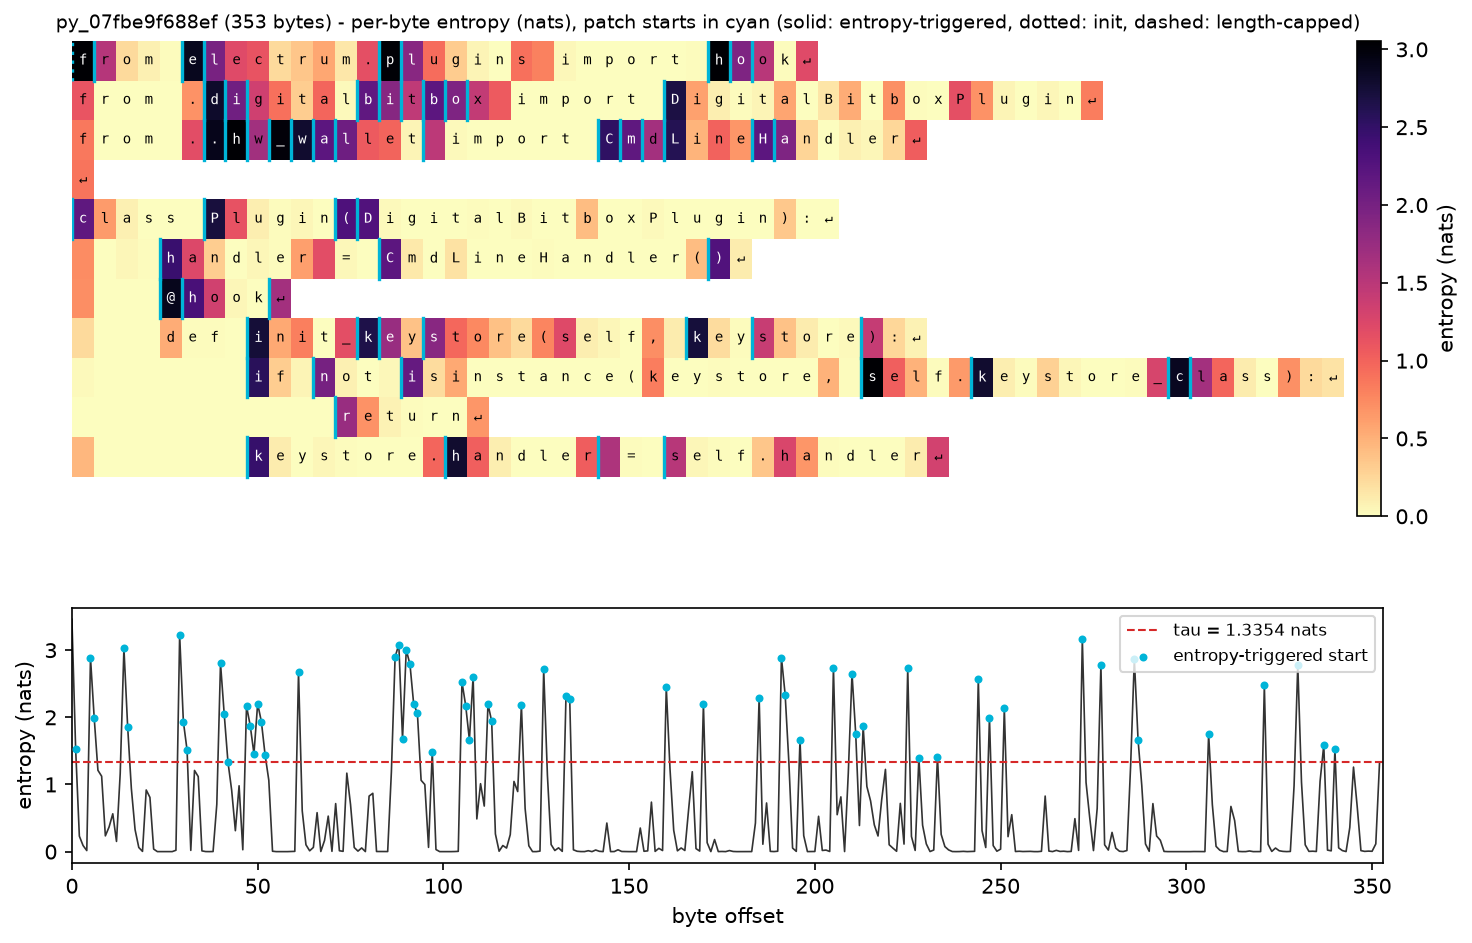
\includegraphics[width=\linewidth]{../../results/figures/stream_a/swa512-float32-t1.3354-mplnone-91aa6b8e/entropy_heatmap_py_07fbe9f688ef.png}
\end{columns}
\end{frame}

\section{Stream B: data and ground truth}
\begin{frame}{Stream B: corpus, targets and controls}
\begin{itemize}\small
\item \nSamples{} hash-verified files: 8{,}000 Python functions (CodeSearchNet), 8{,}000 C++ files (The Stack; CodeSearchNet has no C++), 300 WikiText-103 paragraphs; calibration \nCalPy{}/\nCalCpp{}/\nCalEn{}, test \nTestAll{}.
\item Targets: \hl{tree-sitter} constituent starts (Python, C++), \hl{benepar} parses (English); character offsets round-tripped to UTF-8 bytes; unique non-wrapper starts, outermost node wins.
\item Structure-blind baselines from the same bytes: newline, indentation change, word start.
\item O4 noise set: \OFourRate{} of lines or keywords, \OFourCaseRate{} of identifiers; rebuilt at 5--40\% for the rate sweep.
\item O5 regions: tree-sitter queries for \texttt{*}, \texttt{\&}, \texttt{new}, \texttt{delete}; audit reproduced \xAuditRepro{} regions, an independent labeller agreed on \xAuditAgree{} statements.
\item Extension data: a disjoint 29k-file distillation corpus (pinned revision) and the pre-registered English holdout (\xHoldFiles{} paragraphs from 120 unused articles).
\end{itemize}
\end{frame}

\section{Stream C: statistics}
\begin{frame}{Ground truth from parsers: interactive tree views}
\begin{itemize}
\item \textbf{Code:} tree-sitter gives an exact grammar tree; the highlighted nodes are the constituents we keep as targets (statement- and expression-level) with their start and end bytes.
\item \textbf{English:} benepar gives a predicted phrase tree (NP, VP, PP); targets are phrase starts.
\item Each viewer shows the full parse tree next to the source, as a self-contained HTML page (no server, no network).
\end{itemize}
\vspace{2mm}
\textbf{Open a view} (links work when the PDF is opened from the repository):\\[1mm]
\href{../../../stream_b/tree_views/py_a1567fe2419b.html}{Python} \quad
\href{../../../stream_b/tree_views/cpp_362b99d47547.html}{C++} \quad
\href{../../../stream_b/tree_views/prose_504f378c8948.html}{English}\\[1mm]
{\footnotesize Viewers: \texttt{stream\_b/tree\_viewer.py}, \texttt{stream\_b/prose\_tree\_viewer.py}; examples in \texttt{stream\_b/tree\_views/}.}
\end{frame}

\begin{frame}{Stream C: frozen protocol}
\begin{itemize}
\item One-to-one matching within $k$ bytes; $k\in\{0,1,2,4,8\}$ chosen on the \hl{calibration split only} $\rightarrow$ $k=0$ everywhere.
\item Fixed-EOF null keeps patch-length multiset and boundary count; paired file bootstrap (\nBoot{}).
\item Frozen teacher run scored once; later test-file runs (student, $\tau^*$, $k=1,2$, O4 sweep, HF full attention, $\tau$ grid) \hl{selected nothing}.
\item New checks: repository-clustered bootstrap (Python, \xRepoN{} repos) widens the CI \xRepoWiden{}$\times$ to \xRepoCI{}; parser error recovery (\xErrShare{} of C++) changes the margin by \xErrDiff{} \xErrDiffCI{}; files $>$8{,}191 bytes by \xLongDiff{} \xLongDiffCI{}.
\end{itemize}
\end{frame}

\section{Results}
\begin{frame}{P1: real alignment, but not beyond line/word segmentation}
\centering\small
\begin{tabular}{lrrrrl}
\toprule
& F1 & $H_0$ F1 & $\Delta$ [95\% CI] & F1/$H_0$ & vs.\ best baseline \\
\midrule
Python & \FonePy{} & \FoneNullPy{} & \MarginPy{} \MarginCIPy{} & \xRatioPy{}$\times$ & \VsBasePy{} (\StrongestPy{}) \\
C++ & \FoneCpp{} & \FoneNullCpp{} & \MarginCpp{} \MarginCICpp{} & \xRatioCpp{}$\times$ & \VsBaseCpp{} (\StrongestCpp{}) \\
English & \FoneEn{} & \FoneNullEn{} & \MarginEn{} \MarginCIEn{} & \xRatioEn{}$\times$ & \VsBaseEn{} (\StrongestEn{}) \\
\bottomrule
\end{tabular}
\vspace{1em}
\begin{itemize}
\item P1 \hl{supported} against the null ($p\le10^{-4}$ everywhere); against the best structure-blind baseline BLT \RTwoAll{}.
\item At BLT's density F1 is capped at $2/(r{+}1)$ = \xFoneCapPy{} / \xFoneCapCpp{} / \xFoneCapEn{}; density-free check: word starts beat BLT on \hl{both} precision and recall (Py \xWordPPy{}/\xWordRPy{} vs.\ \PrecPy{}/\RecPy{}).
\item Precision $\ll$ recall (proposal predicted the reverse): every boundary has $\ge e^{\tau}\approx3.8$ live continuations; identifier interiors are flat but not syntactic.
\item P2 \hl{supported}: end margins \EndMarginPy{}, \EndMarginCpp{}, \EndMarginEn{}.
\end{itemize}
\end{frame}

\begin{frame}{P3 reversed --- prose constituents start at words}
\begin{itemize}
\item Predicted: prose near chance. Observed: prose margin \MarginProse{} $>$ code \MarginCode{}.
\item Benepar constituents begin at words; the word-start rule alone gets \StrongestFoneEn{} F1 in English.
\item F1/$H_0$ = $R/R_0$ is capped at $1/R_0$ $\approx$ mean patch length (\xRatioCapPy{} / \xRatioCapCpp{} / \xRatioCapEn{}), so its \xRatioPy{}$\times$ / \xRatioCpp{}$\times$ / \xRatioEn{}$\times$ favours code mechanically.
\item Chance-corrected recall $(R-R_0)/(1-R_0)$ ranks \hl{English first}: \xKappaEn{} vs.\ \xKappaPy{} (Py), \xKappaCpp{} (C++).
\item BPP variance half of P3 holds: within-file variance \BppVarCpp{} (C++), \BppVarPy{} (Py) vs.\ \BppVarEn{} (En).
\end{itemize}
\end{frame}

\begin{frame}{P4 reversed at the start byte --- confirmed at the forced bytes}
\begin{columns}[T]
\column{.52\textwidth}\small
\begin{itemize}
\item Per-type mean start margin: forced \DetMarginPy{} vs.\ open \OpenMarginPy{} (Py) --- opposite of P4.
\item Test: boundary rate at bytes \emph{after} $s$, same null draws (start rows \xPosCheck{} the frozen recalls).
\item Rest of keyword: \xKwDetPy{} (Py), \xKwDetCpp{} (C++) vs.\ null.
\item Byte after keyword: rate \xPostKwRateDetPy{} (Py), \xPostKwRateDetCpp{} (C++) vs.\ null \xOffNullPy{} (Py) / \xOffNullCpp{} (C++); open-ended stays at the null.
\item Boundary returns where choice reopens: Python condition start (rate \xNextRateDetPy{}); C++ after the forced \texttt{(} (rate \xOffDetCppIV{}).
\item \hl{Forcing is real; the start byte is just before it.}
\end{itemize}
\column{.48\textwidth}
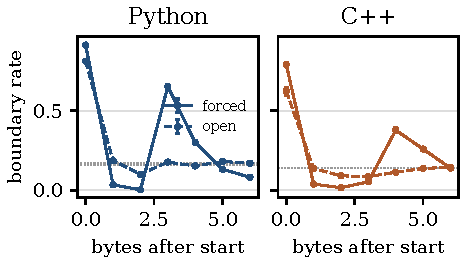
\includegraphics[width=\linewidth]{generated/p4_offsets.pdf}
\end{columns}
\end{frame}

\begin{frame}{O3: depth on a common scale}
\centering
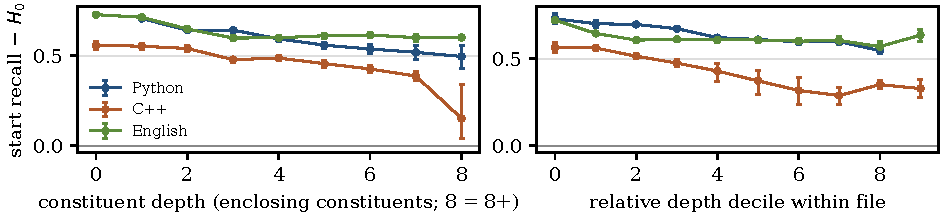
\includegraphics[width=.95\textwidth]{generated/depth_normalised.pdf}
\begin{itemize}\small
\item Raw tree-sitter depth counts language-specific scaffolding $\rightarrow$ count enclosing \emph{constituents} instead, and normalise within file.
\item Largest at the outermost constituents; 1 $\rightarrow$ 7 enclosing constituents: Py \xDepthOnePy{} $\rightarrow$ \xDepthSevenPy{}, C++ \xDepthOneCpp{} $\rightarrow$ \xDepthSevenCpp{}, En \xDepthOneEn{} $\rightarrow$ \xDepthSevenEn{}. Python $>$ C++ at every depth.
\end{itemize}
\end{frame}

\begin{frame}{O4: noise, now as a rate sweep}
\centering
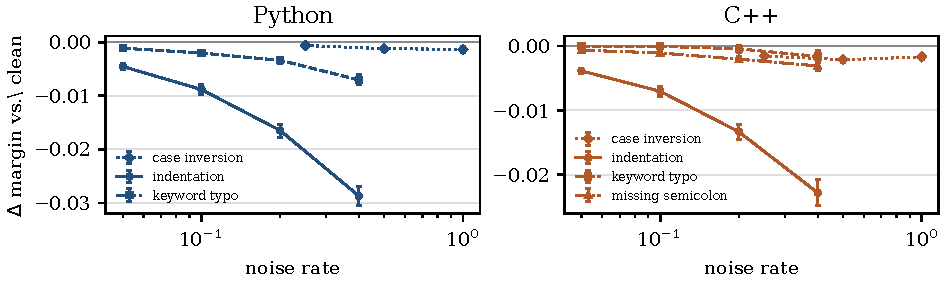
\includegraphics[width=.95\textwidth]{generated/o4_sweep.pdf}
\begin{itemize}\small
\item Same \xOFourSweepFiles{} held-out files per language, each noise type at 5--40\% (case 25--100\%).
\item Indentation does by far the most damage (Py \xOFourIndentLoPy{} $\rightarrow$ \xOFourIndentHiPy{}, C++ \xOFourIndentLoCpp{} $\rightarrow$ \xOFourIndentHiCpp{}); the others also grow with rate but stay small (typos \xOFourTypoHiPy{} / \xOFourTypoHiCpp{}, semicolons \xOFourSemiHiCpp{} at 40\%). Typos cut BPP (\xOFourTypoBppPy{} / \xOFourTypoBppCpp{}). Every margin $\ge$ \xOFourSweepMinMargin{}.
\end{itemize}
\end{frame}

\begin{frame}{O5: no evidence of risk-aware compute near memory-unsafe code}
\begin{itemize}
\item Label audit: \xAuditRepro{} regions reproduced; independent lexical labeller agrees on \xAuditAgree{} statements.
\item Frozen coefficient \xOFiveFull{} \xOFiveFullCI{} boundaries/byte --- but:
\item File FE only: \hl{\xOFiveRaw{} \xOFiveRawCI{}} --- unsafe statements get \emph{fewer} boundaries (more predictable identifiers).
\item Positive only after conditioning on identifier entropy; size \xOFiveRel{} of the mean, \xOFiveVsIdent{} of a 1-SD identifier-entropy effect.
\item Inverse BPP with file FE only: \xOFiveRawBpp{} \xOFiveRawBppCI{} (null).
\item Reading: a small conditional effect, not risk awareness.
\end{itemize}
\end{frame}

\section{Extension}
\begin{frame}{Beyond the proposal: a 7$\times$ smaller distilled patcher}
\centering\small
\begin{tabular}{lrrrl}
\toprule
& Teacher $\Delta$ & Student $\Delta$ & kept & Student$-$teacher [95\% CI] \\
\midrule
Python & \MarginPy{} & \xStuMarginPy{} & \xStuRetainPy{} & \xStuDiffPy{} \xStuDiffCIPy{} \\
C++ & \MarginCpp{} & \xStuMarginCpp{} & \xStuRetainCpp{} & \xStuDiffCpp{} \xStuDiffCICpp{} \\
English & \MarginEn{} & \xStuMarginEn{} & \xStuRetainEn{} & \xStuDiffEn{} \xStuDiffCIEn{} \\
\bottomrule
\end{tabular}
\begin{itemize}\small
\item Online KD ($\alpha=0.1$, $T=2$) on a disjoint 29k-file corpus; val boundary F1 vs.\ teacher \xDistFone{}; no-teacher control ($\alpha=1$) \xAlphaFone{}.
\item Full 16{,}300-file extraction + frozen C-v1 scoring with its own calibration ($k=0$).
\item Native teacher minus teacher on 512-byte windows: \xTfiveDiffPy{} (Py) / \xTfiveDiffCpp{} (C++) F1, \xTfiveSharePy{} / \xTfiveShareCpp{} of the student's deficit; capacity explains the rest.
\item Cost: forward \xEffForward{}$\times$ faster than the teacher on a \xEffGpu{}.
\end{itemize}
\end{frame}

\begin{frame}{Follow-ups: byte-balanced student, adapted teacher}
\centering\small
\begin{tabular}{lll r}
\toprule
& Balanced$-$student [95\% CI] & Adapted$-$student [95\% CI] & bar \\
\midrule
Python & \xBalDiffPy{} \xBalDiffCIPy{} & \xAdaptDiffPy{} \xAdaptDiffCIPy{} & \xAdaptWidthPy{} \\
C++ & \xBalDiffCpp{} \xBalDiffCICpp{} & \xAdaptDiffCpp{} \xAdaptDiffCICpp{} & \xAdaptWidthCpp{} \\
English & \xBalDiffEn{} \xBalDiffCIEn{} & \xAdaptDiffEn{} \xAdaptDiffCIEn{} & \xAdaptWidthEn{} \\
\bottomrule
\end{tabular}
\begin{itemize}\small
\item Paired $\Delta$ differences, $k=0$, on the pre-registered 600-file code subset and the \xArmsNEn{} English test files (exploratory: full-corpus extraction did not fit).
\item Byte-balanced sampling trades code for prose: English up, code slightly down; window F1 vs.\ teacher \xBalWinFone{} (distilled \xBalRefWinFone{}).
\item Adapted teacher (99.5M, same loss and data): window F1 \xAdaptWinFone{}; pre-registered verdict \hl{\xAdaptVerdict{}} (\xAdaptWins{} of 3 domains beat the student's CI width).
\item In code it matches the unadapted teacher read through the same windows: it recovers the teacher rather than improving on it.
\end{itemize}
\end{frame}

\begin{frame}{Threshold sweep and the confirmatory English holdout}
\centering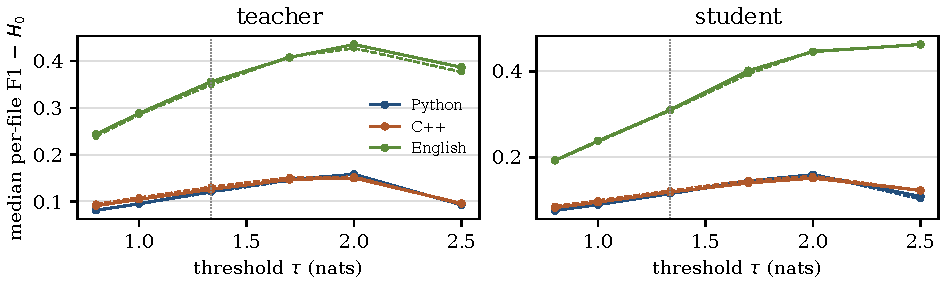
\includegraphics[width=.92\linewidth]{generated/tau_sweep.pdf}
\footnotesize
\begin{itemize}
\item Pre-registered $\tau^*$ on calibration: teacher \xTauStarTeacherPy{}; student \xTauStarStudentPy{}/\xTauStarStudentCpp{}/\xTauStarStudentEn{}.
\item One test run at $\tau^*$: teacher $\Delta$ \xTauConfTeacherPy{} (Py), \xTauConfTeacherCpp{} (C++), \xTauConfTeacherEn{} (En) --- still below baselines (\xTauConfVsBaseTeacherPy{}).
\item Student at its own $\tau^*$: $\Delta$ \xTauConfStudentPy{}, \xTauConfStudentCpp{}, \xTauConfStudentEn{} --- also below baselines.
\item Later, exploratory: grid on test (dashed) peaks at the same $\tau^*$ (\xTauTestAgreeTeacher{}/3, \xTauTestAgreeStudent{}/3); every $\tau$ trails the best baseline by $\ge$\xTauTestMinGap{} F1.
\item English holdout (\xHoldFiles{} unseen paragraphs, scored once): teacher \xHoldTeaMargin{}, student \xHoldStuMargin{}; vs.\ word starts \xHoldTeaVsWord{}.
\end{itemize}
\end{frame}

\begin{frame}{Verdict on H1 and the proposal's deliverables}
\begin{itemize}
\item \textbf{Criteria from the proposal:} P1 beats both baselines, P2 holds, P3 dissociates code from prose, P4 stratification appears.
\item \textbf{Outcome:} H1 is \hl{not supported} under this criterion: only P2 holds as stated.
  \begin{itemize}
  \item P1: beats the density-matched null everywhere, but not the whitespace and word-start baselines.
  \item P2: holds (end margins negative).
  \item P3: reversed, also under chance-corrected recall.
  \item P4: reversed at the start byte; the mechanism holds at the bytes after the keyword.
  \item Precision $>$ recall (proposal's mechanism): fails.
  \end{itemize}
\item \textbf{Deliverables:} (1) extraction pipeline \texttt{stream\_a}; (2) tree-sitter / benepar mapping with memory-unsafe queries \texttt{stream\_b}; (3) harness with P1--P4, both baselines, permutation test, depth and type stratification \texttt{escape\_scoring}, \texttt{escape\_eval}; (4) entropy heatmaps and BPP profiles; (5) report and these slides.
\item \textbf{Released models:} \href{https://huggingface.co/Devatri/escape-blt-entropy-student}{student}, \href{https://huggingface.co/Devatri/escape-blt-entropy-student-alpha1}{no-teacher control ($\alpha{=}1$)}, \href{https://huggingface.co/Devatri/escape-blt-entropy-student-balanced}{byte-balanced student} on Hugging Face; checkpoints and curves in the \href{https://forge.coreweave.com/wandb/kanhadivyansh123-iiit-hyderabad/escape-blt-patching}{W\&B project}.
\end{itemize}
\end{frame}

\begin{frame}{Limitations and future work}
\begin{itemize}
\item \textbf{Limitations:} third-party checkpoint with a restored window (no bitwise check against the gated original); English targets are predicted parses; O5 labels are syntactic; one student size, one seed; follow-up arms scored on a subset; no subword-tokenizer baseline for O4; no multiple-comparison correction; English intervals resample paragraphs, not articles.
\item \textbf{Future work:} parser-supervised teacher; subword baseline for O4; several student seeds; full-corpus scoring of the follow-up models; single-pass student kernel; bitwise comparison with the original checkpoint.
\end{itemize}
\end{frame}

\begin{frame}{Conclusions}
\begin{itemize}
\item Entropy boundaries track constituent starts \hl{\xRatioEn{}--\xRatioPy{}$\times$ above chance} --- held-out and on the English holdout; a 7$\times$ smaller student keeps $\approx$90\% of the margin.
\item They do \hl{not} beat indentation / word-start segmentation at any $\tau$ or $k$.
\item Each failed prediction has a mechanical explanation:
  \begin{itemize}
  \item precision $<$ recall: several boundaries per target;
  \item P3: prose constituents begin at words, where the patcher fires;
  \item P4: forcing acts after the opener, not at its start;
  \item O5: the ``residual'' appears only after an identifier-entropy control.
  \end{itemize}
\item Entropy is a genuine but shallow signal of word and line onsets --- syntax shapes it without being what it measures.
\end{itemize}
\end{frame}
\end{document}
